\documentclass[11pt,singleside]{myfithesis2}
\usepackage[hyphens]{url}
\usepackage[english]{babel}  %  package  for  multilingual  support
\usepackage[utf8]{inputenc}  %  UTF-8  encoding
\usepackage[IL2]{fontenc}
\usepackage[plainpages=false,pdfpagelabels,unicode]{hyperref}
\usepackage{fancyvrb}
\usepackage{graphicx}
\usepackage{listings}
\usepackage{color}
\usepackage{textcomp}
\usepackage[small]{caption}
\usepackage{subcaption}
\usepackage{float}
\usepackage{verbatim}
\usepackage{pdfpages}
\usepackage{cleveref}[2012/02/15]
 
\definecolor{listinggray}{gray}{0.9}
\definecolor{lbcolor}{rgb}{0.9,0.9,0.9}
\definecolor{darkgray}{gray}{0.3}
\definecolor{palegray}{gray}{0.85}

\hyphenation{YSoft SafeQ Sikuli Soft}

\lstset{
	numbers=left,
	backgroundcolor=\color{lbcolor},
	tabsize=4,
	rulecolor=,
	language=java,
       basicstyle=\footnotesize,
       %basicstyle=\ttfamily,
       upquote=true,
       aboveskip={\baselineskip},
       %belowskip={\baselineskip},
       columns=fixed,
       showstringspaces=false,
       extendedchars=true,
       breaklines=true,
       prebreak = \raisebox{0ex}[0ex][0ex]{\ensuremath{\hookleftarrow}},
       frame=tb,
       showtabs=false,
       showspaces=false,
       showstringspaces=false,
       identifierstyle=\ttfamily,
       keywordstyle=\color[rgb]{0,0,1},
       commentstyle=\color[rgb]{0.133,0.545,0.133},
       stringstyle=\color[rgb]{0.627,0.126,0.941},
	emph=, emphstyle=\color{black},
	captionpos=b,
}



\newcommand{\pict}[4]{
	\begin{figure}[h!]
  		\vspace{-7px}
  		\centerline{\fcolorbox{darkgray}{palegray}{\includegraphics[#3]{#2}}}
  		\caption{#1}
  		\label{#4}
	\end{figure}
}

\newcommand{\twopict}[9]{
	\begin{figure}[h!]
  		\vspace{-7px}
		\begin{subfigure}{.5\textwidth}
  			\centerline{\fcolorbox{darkgray}{palegray}{\includegraphics[#8]{#2}}}
  			\caption{#1}
  			\label{#3}
		\end{subfigure}
		\begin{subfigure}{.5\textwidth}
  			\centerline{\fcolorbox{darkgray}{palegray}{\includegraphics[#8]{#5}}}
  			\caption{#4}
  			\label{#6}
		\end{subfigure}
		\caption{#7}
		\label{#9}
	\end{figure}
}

\crefformat{footnote}{#2\footnotemark[#1]#3}

\makeatletter
\renewcommand\paragraph{
   \vspace{-10pt}
   \@startsection{paragraph}{4}{0mm}
      {\baselineskip}
      {- 5pt}
      {\normalfont\normalsize\bfseries}
}
\makeatother
\renewcommand\lstlistingname{Source code}
\renewcommand\lstlistlistingname{List of source codes}

\hypersetup{
    colorlinks,
    citecolor=black,
    filecolor=black,
    linkcolor=black,
    urlcolor=black
}

\clubpenalty=10000
\widowpenalty=10000
\thesistitle{Making Internal Communication in~a~Software Company More~Efficient}  %  thesis  title
\thesissubtitle{Master's Thesis}
\thesisstudent{Bc. Martin Bryndza}        %  name  of  the  author
\thesiswoman{false} %  defines  author’s  gender
\thesisfaculty{fi}
\thesisyear{2015}
\thesisadvisor{Mgr. Peter Neugebauer, MBA}  %  fill  in  advisor’s  name
\thesislang{en} %  thesis  is  in  English
\begin{document}
\FrontMatter
\ThesisTitlePage
\begin{ThesisDeclaration}
\DeclarationText
\AdvisorName
\end{ThesisDeclaration}
\begin{ThesisThanks}
I would like to thank to my supervisor Mgr. Petr Neugebauer, MBA for his valuable advices and guidance. Great thanks go to the Y Soft Corporation for giving me the opportunity to perform the unnecessary research. Many thanks also go to my colleagues from the ETNA team, who contributed to this thesis with their cooperation and willingness to try new things. These are the people who agreed to do some extra work without hesitation. I would like to send many thanks also to my colleagues from the QA team for their support in the last months of me working on this thesis. With their help I was able to have enough time for the thesis while also getting all the planned work done for each sprint. Last but not least, I would like to thank to my dear Marie for her love and patience she had with me working overnight and also to my parents for their support throughout my studies. 
\end{ThesisThanks}
\begin{ThesisAbstract}
The goal of this thesis is to streamline communication between teams and their members and to prevent loss of productivity due to frequent interruptions in a mid-size software company, where employers are dealing with adaptation of agile approaches. The thesis should analyze internal processes as well as requirements and expectations of different stakeholders regarding productivity, especially communication gaps. Based on these identified issues, the implementation part of the work will cover design and implementation of a tool, which will enforce the team members to follow the proposed process(es). This thesis is realized in cooperation with Y Soft Corporation, a.s.
\end{ThesisAbstract}
\begin{ThesisKeyWords}
Agile, Communication, Company, Internal, Interruption, Java, Organization, Pomodoro, Spring, Team, Teamwork, Thymeleaf.
\end{ThesisKeyWords}
\MainMatter
\tableofcontents %  prints  table  of  contents
%\listoffigures % prints list of pictures
%\lstlistoflistings % prints list of blocks of code
%\listoftables % prints list of tables

\chapter{Introduction}
In recent years, word Agile became very popular among managers in software companies. As many other companies, development in Y Soft has become agile as well. After several struggles in the beginning, the company has managed to tailor Scrum framework to its needs and the employees has got used to the new style of work.

Agile software development is driven by The Agile Manifesto \cite{agileManifesto}, which consists of the following four principles:
\begin{itemize}
	\item Individuals and interactions over processes and tools
	\item Working software over comprehensive documentation
	\item Customer collaboration over contract negotiation
	\item Responding to change over following a plan 
\end{itemize}
The second principle results in less robust documentation, which means that a lot of knowledge is kept by the people only. Obtaining that knowledge by somebody else brings in a need to communicate. Following the last point of the manifesto, everything around products can change rapidly and so does the knowledge, which has to be distributed again. This brings up a need for more and more communication. 
(Since 2001, when the manifesto was written, software products became much more complicated and interconnected. Such systems require lots of cooperation not only inside teams, but also among them. This makes communication a significant part of a day of every software engineer.)


	\section{Motivation}
Several months ago, as a Junior Quality Assurance Engineer in Y Soft, I've become a part of an engineering team. My role now is to give support to the team throughout the development cycle, in terms of assuring high level of quality. To be able to do that, I have to give inputs and tightly cooperate with the team all the time. 

After a few weeks of my presence in the team I started noticing, that the developers of the team go home frustrated quite regurarly. Often they leave work earlier. Their reason is that they made no progress that day and there is no point in staying there longer. On the other hand, some other days I see them working late hours, most of the time apparently stressed out about not meeting deadlines.

In Y Soft, we use a tailored Scrum framework. This means, that as a team member, I'm also part of planning and team review meetings. There I noticed, that only about half of the developers' time is planned. Despite of that, there is a serious amount of time pressure at the end of the sprint, in order to meet the planned sprint goals on time. Sometimes, some goals even have to be moved to the next sprint.

This got me thinking, why is that so. What it is that the developers are doing, which is not planned. I don't see them procrastinating much and they very rarely take breaks. In fact, it was not very difficult to tell, that it is the communication, which is on a high level in the Research and Development department. Some of the communication, like corporate meetings or cooperation on tasks, is predicted and planned. But there also is a significant amount of unpredictable communication, which can be denoted as unofficial. This includes ad-hoc help to colleagues with their tasks, providing information when requested, conversations about long term goals, about state of things, sharing feedbacks and more. These conversations are not managed nor tracked, they can happen anytime and take several minutes or maybe even hours each day.

I asked my colleagues to give their opinions on this observation. Almost all of them confirmed, that the internal communication is distractive for them and that they feel its direct impact on their productivity. The other inquired colleagues declared, that they are only rarely interrupted or that they don't mind the interruptions. If an interruption is related to their current task, it is mostly not seen as interruption at all.

The aforementioned realization and research are reasons for this thesis. The main goal is to streamline the internal communication between team members in Research and Development department in Y Soft Corporation, a.s., with possible applicability also to other departments and companies. The main focus will be on the daily communication, that happens throughout the Scrum Process. The focused part of the process is marked with a red arrow on Figure \ref{pic:scrumProcess}.

\pict{Scrum Process \cite{scrumProcess}}{data/Scrum_process.png}{width=0.8\textwidth}{pic:scrumProcess}


	\section{Structure of the Thesis}
The first part of this thesis explains what it means for a software engineer to be interrupted. Several studies are mentioned in this chapter, in order to get an image of all possible impacts that interruptions can have. The impacts are significant not only for an engineer, but a knowledge worker in general. Rest of this chapter is dedicated to the three most common time management techniques. One of the techniques is chosen as the most appropriate for use in an agile environment, where cooperation is essential.

Chapter \ref{internalCommunication} introduces a concept of the internal organizational communication, mentioning several most common myths in communication management. Second part of this chapter advises on the steps to take and risks to count with, when establishing an efficient internal communication. This is followed by some ideas on why it would not be a good idea to eliminate ad-hoc face-to-face communication in an agile environment, as this would be the simplest solution of the aforementioned issues.

Analytical part of the thesis focuses on the historical background and current state of the Y Soft Corporation, as it is essential for understanding the nature of communication in the company. There it is possible to see the rapid growth in number of employees in the recent years, which introduced the issues this theses is addressing. Report from an unconference with Kentico Software is also a part of this chapter, which confirmed that Y Soft's employees are not the only ones who are troubled by frequent interruptions in their work. The chapter is concluded by definition of issues, that need to be resolved.

The final parts of the thesis bring a solution in a form of a new tool. The usage instruction of the tool are included in this part, together with a list of issues this tool solves and purposes it can serve. From the development point of view, used technologies, architecture and design patterns are presented here. The chapter also includes the feedback from colleagues that were using the tool, as well as the one that performed a code review.

The thesis also includes summarization of results in terms of measured improvements as well as subjective feelings of the users. The last chapter is dedicated to ideas about future development of the tool and its potential.


\chapter{Effective Work}

This chapter will give you an insight on what an interruption means to a software engineer. The reasoning will be supported with a few researches bringing interesting results of the real cost of interruptions. In the second part, you can find a short summary of The Pomodoro technique, which can help reducing interruptions and boosting up productivity. The section also contains a list of objectives, that are necessary, in order to implement the technique into your work customs.

	\section{The Cost of Interruptions}

		\subsection{What It Means To Interrupt a Software Engineer}
In a company, there are positions, for which interruptions are just a normal part of the day. Sometimes, interruptions are what their work is mostly based on. A nice representation of this group are managers, who constantly change focus throughout the day. Their time is usually spit up in one hour intervals, each of them containing a single task. Likewise, if we take people from marketing. An interruption for them means a time spent dealing with the interruption and a few seconds more to find out where they had finished. For software engineers, it is much more different.

A comic made by Jason Heeris [Appendix \ref{app:software engineer}],  is probably the best way to give you an idea about what it means for a software engineer to be interrupted.\footnote{Erik Dietrich in an article on his blog \cite{costOfInterruptions} provides a simple way of showing, what it means for a programmer to be interrupted: Write down a series of 3 to 4 digit numbers in a sequence. Now, tell a person to add those numbers as fast as possible without writing anything down. After some time, ask the person questions about how it is going, what number he/she is currently adding, whether it is 198 or 674 and get him/her to respond. Ask him to help you with adding some other three numbers real quick. Moreover, you can pretend a phone call in the vicinity of the person, talking about some numbers. When the person is done, check the result and ask, how many times a fresh start was necessary. Several experiments, which I have performed on my friends, showed, that usually the examinee had to start over several times and also did not get the correct result.} Software engineers often find it very difficult to start where they had finished prior to the interruption, if it is at all possible. As an example, debugging of code may become a very time demanding process, which requires a high level of concentration, as there is no undo or step backwards. A distraction may cause that the engineer makes a mistake, forgets the context or the debugged program times out and terminates itself. This can cause frustration and a nontrivial loss of time.

%Imagine a software engineer in a middle of a debugging task. He has finally come to a sufficient level of understanding of the tricky condition in the code, has done the right amount of cycles to get the correct value in a variable, which purpose is a little mystery to him, and is very probably just about to find out, what causes the exception, that the important customer sees in logs from time to time under unknown conditions. All of a sudden, a colleague comes by to ask about that other task the software engineer had been working on and is currently under test. The distraction causes him to accidentally step over the expression instead of stepping into it. So, he asks the colleague to repeat the question, as he was only partly listening. After helping the colleague, he looks down at his paper wondering, what ''18rts97'' means, and restarts the debugging process.


		\subsection{The Real Cost of Interruptions }\label{costOfInterruptions}
Several studies \cite{studySpeedAndStress, studyAttention, studyDealingWithInterruptions, studyResumptionStrategies} have been done on interruptions and their impact on work. Various measures have been done including context of the interruptions, their frequency, impact on work efficiency, stress level, workload and effort. Other studies focus on the amount of productivity time wasted by these interruptions. In this section, I will mention several of these studies.

\paragraph*{More Speed and Stress: } The study \cite{studySpeedAndStress} was performed on people answering to emails in their inbox as quickly, correctly and politely as possible. They were told that their ``supervisor'' is sitting in another room and will contact them regularly to ask questions either over telephone or IM\footnote{IM can refer to Instant Messenger or Instant Message, which is a text message sent using a service (messenger), that enables real time communication over the Internet.}. The results of the study show, that when people are constantly interrupted, they develop a mode of working faster and producing less, to compensate for the time lost by the interruptions. However, this faster pace of work has its cost: higher workload and frustration, more stress, effort and time pressure. In conclusion, when being interrupted, the work can be done faster, but at a price. This study also shows that the context of the interruption to the currently performed task makes no difference or a very little difference. Table \ref{table:workload} shows the measures stated.
\begin{table}[h]
\centering
\resizebox{\textwidth}{!}{%
\begin{tabular}{|l|r|r|r|r|r|}
\hline
                           & \textbf{Mental workload} & \textbf{Stress} & \textbf{Frustration} & \textbf{Time pressure} & \textbf{Effort} \\ \hline
\textbf{No interruptions}  & 10.02                    & 6.92            & 4.73                 & 11.02                  & 9.50            \\ \hline
\textbf{Same context}      & 10.83                    & 9.46            & 6.63                 & 12.69                  & 11.04           \\ \hline
\textbf{Different context} & 11.50                    & 9.13            & 6.48                 & 12.17                  & 11.52           \\ \hline
\end{tabular}
}
\caption{Mean workload measures across interruption types. Scale is 1(low)-20(high).}
\label{table:workload}
\end{table}
\paragraph*{The Cost of Not Paying Attention: } This study \cite{studyAttention} is focusing on the amount of time that interruptions waste. Data were gathered by observers in real offices, where these observers noted every single change of action of a knowledge worker\footnote{A knowledge worker is anyone who works for a living at the tasks of developing or using knowledge. \cite{knowledgeWorker}}. Their findings are, that interruptions consume 28 \% of the knowledge worker's day. Not all of these interruptions are unnecessary and considered as a waste of time. For example, helping a co-worker in a business-related matter is recognized as beneficial to the company's well being. Nevertheless, combining the unnecessary interruptions and the time needed to switch context results in 503.52 hours per employee per year. The study also mentions common ways of how workers fight constant interruptions in order to get their work done. Some of them are: \label{list:avoidingCommunication}
\begin{itemize}
	\item refuse eye contact;
	\item post a sign;
	\item work, when no one else is around;
	\item relocate to another office or conference room;
	\item work from home;
	\item work offsite.
\end{itemize}
These methods clearly disrupt teamwork or are at least not beneficial to it. Some of them are also quite ineffective and could be ignored by co-workers.
\paragraph*{Dealing with interruptions: } This older study \cite{studyDealingWithInterruptions} used 29 hours of videotaped materials to perform a diary research. Their findings are, that participants, on average, experienced over four interruptions per hour. Moreover, 41 \% of the time, the disrupted task was not resumed after the interruption finished. It is presumed that the worker does not return to the previous task either because it is too difficult to resume the task from the point it had been disrupted, or the task has been forgotten. Furthermore, the study points out a benefit that recipients receive when being interrupted, and the service that individuals may be contracted to perform for others.
\paragraph*{Resumption strategies for interrupted programming tasks: } Another study \cite{studyResumptionStrategies} performed on 10,000 recorded sessions of 86 programmers and surveyed 414 other programmers. The results say that resumption is a frequent and persistent problem. Only 10 \% of the sessions have programming activity resumed in less than 1 minute and only 7 \% of the programming sessions involve no navigation to other locations prior to resuming work. Actually, about 30 \% of sessions took more than 30 minutes to restore the programming task.

In conclusion, constant interruptions are mostly harmful to the work efficiency, ease of work and company itself. On the other hand, some of the interruptions are highly beneficial to the interrupting person and the interrupted worker as well. Most of the common techniques used to avoid unwanted interruptions are really basic, mostly inefficient and disruptive to the teamwork.

	\section{Productivity Techniques}
Internet, as well as libraries are full of books, papers and articles about work productivity. The proposed solutions wary from a set of simple roles to complex techniques. However, two of the techniques stand out, as they are supported by a big user base - Pomodoro Technique \cite{pomodoro} and Getting Things Done \cite{gtd}. The Pomodoro Technique was created with the aim of using time as a valuable ally to accomplish what we want to do, the way we want to do it, and to empower us to continually improve our work or study processes. This technique is often used complementary to a set of methods named ''Getting Things Done'' created by David Allen, which he presents as ''A gold mine of insights for how to have more energy, be more relaxed, and get a lot more accomplished with much less effort.''	
	
The Getting Things Done is more of a personal guide for organizing tasks into projects in order to stop forgetting to do things, to make yourself do them, to do them on time and to have more time for yourself. The method is suited more for a solitary workers, who do not need to work in teams or the teamwork is not very intense, as the method does not consider external interruptions. On the other hand, The Pomodoro Technique requires much less administration and focuses more on actually doing the things. It also fights interruptions while not dismissing them completely, which makes it more suitable for purposes of this thesis.

	\section{The Pomodoro Technique}
%The Pomodoro Technique was invented by Francesco Cirillo in the early 80s, as a result of his own and fellow students ineffective study habits. The name ''Pomodoro'' translates as ''Tomato'' and is inspired by a kitchen timer, that usually comes in a shape of this vegetable. And it is this kitchen-timer-like device which plays an important role in the process of using the Pomodoro Technique.

The goal of the Pomodoro Technique is to provide a simple tool/process for improving productivity of not only individuals, but also whole teams. According to \cite{pomodoro}, the technique is supposed to do the following:
\begin{itemize}
	\item alleviate anxiety linked to becoming\footnote{Becoming is an abstract, dimensional aspect of time which is supported by the idea of representing time on an axis,  as we would represent spatial dimensions. This results in a concept of the duration of an event and the idea of being late (the distance of two points on the temporal axis). \cite{pomodoro}};
	\item enhance focus and concentration by cutting down on interruptions;
	\item increase awareness of your decisions;
	\item boost motivation and keep it constant;
	\item bolster the determination to achieve your goals;
	\item refine the estimation process, both in qualitative and quantitative terms;
	\item improve your work or study process;
	\item strenghten your determination to keep on applying yourself in the face of complex situations.
\end{itemize}

Francesco Cirrillo in \cite{pomodoro}, founded the Pomodoro Technique on three basic assumptions:
\begin{itemize}
	\item A different way of seeing time (no longer focused on the concept of becoming) alleviates anxiety and in doing so leads to enhanced personal effectiveness. 
	\item Better use of the mind enables us to achieve greater clarity of thought, higher consciousness, and sharper focus, all the while facilitating learning. 
	\item Employing easy-to-use, unobtrusive tools reduces the complexity of applying the Technique while favoring continuity, and allows you to concentrate your efforts on the 	activities you want to accomplish. Many time management techniques fail because they subject the people who use them to a higher level of added complexity with respect to the intrinsic complexity of the task at hand.
\end{itemize}

The following objectives are required to be met, one after another, in order to implement the Pomodoro Technique \cite{pomodoro}.
\paragraph*{Find out how much effort an activity requires: } First, a To Do Today Sheet should be created out of a pool of tasks in an Activity Inventory Sheet, which contains all the tasks ordered according to their priority. The traditional Pomodoro takes 25 minutes of work and a 5-minute break. When a Pomodoro is started, it ought not to be interrupted by anybody and anything, otherwise it is considered void. The remaining time should always be clearly visible. When Pomodoro rings, it is not allowed to continue working any longer and the current activity is considered finished, at least temporarily. The successfully finished Pomodoro is marked with an X on the To Do Today Sheet. A 3-5 minute break follows, which gives time needed to ``disconnect'' from the activity, assimilate what's been learned and, for example, do something beneficial for health such as stand up and walk around. The whole cycle repeats four times, when a longer 15-30 minute break takes place. The X symbols make it possible to easily measure the total time spent on each activity, which represent the real expended effort.
\paragraph*{Cut down on interruptions: } There are two types of interruptions: internal and external. The internal interruptions are ways to procrastinate on the activity at hand, which generally is a disguised fear of not being able to finish the activity the way we want and when we want. The external interruptions are generally caused by other people. These types of interruptions share the way of dealing with them: invert the dependency on interruptions and make them depend on us. Generally, almost all of these interruptions can be delayed until the end of the currently running Pomodoro or even until later, though the interruption is considered urgent at the time it emerges. The delay isn't usually detrimental to the source of the interruption and gives an enormous advantage in terms of working more effectively. The interruption should be marked on the To Do Today Sheet and the new activity written down in order to be planned based on it's priority at the end of the Pomodoro.
\paragraph*{Estimate the effort for activities: } The long-term objective here is to successfully predict the effort that an activity requires.These estimates are based on the previously finished Pomodoros. The predicted and real number of Pomodoros spent for each activity is noted and used for better predictions in the future.
\paragraph*{Make the Pomodoro more effective and set up a timetable: } These two objectives are implemented after mastering the previous ones. They include using the first and last few minutes of each Pomodoro for reviewing the work done and setting up timetable for each day, in order to prevent working late hours after wasting time in the morning.

\vspace{\baselineskip}
With Pomodoro, there is an ever-valid rule: ''Next Pomodoro will go better.'' According to the Francesco Cirillo's book The Pomodoro Technique \cite{pomodoro}, the technique has been successfully applied in various types of activities: organizing work and study habits, writing books, drafting technical reports, preparing presentations, and managing projects, meetings, events, conferences, and training courses.


\chapter{Internal Communication in an~Organization}\label{internalCommunication}

As defined in \cite{orgCommForSurvival}, an organization is ''an organized collection of individuals working independently within a relatively structured, organized, open system to achieve common goals''. The same publication defines organizational communication as ''the process by which individuals stimulate meaning in the minds of other individuals by means of verbal and nonverbal messages in the context of a formal organization''. Generally, communication maintains and sustains relationships in any organization, and it does not only effect the people communicating at that moment, but also the whole organization as a system.

This chapter will provide you several misconceptions about organizational communication, that are commonly made. The second section contains rules and principles to be implemented in order to improve efficiency of the internal communication. At the end of the chapter, you can find reasonings why ad-hoc face-to-face communication is heart and soul of agile projects.


	\section{Efficiency of Organizational Communication}\label{effOfOrgComm}
There is a common belief that communication is a good thing. It is always beneficial to sit down and talk things through, share thoughts, give opinion, get things straight. And the same common sense tells us, that if a little bit of something is good, more will be better. Since then, managers are widely encouraging people to communicate with their co-workers, subordinates and supervisors. However, little thoughts were given to the way the communication is done, its efficiency and impact on processes. 

A reason why management of many companies is not systematically focused on internal communication is its sudden growth from a small company into an enterprise. Over that time, external communication with customers and partners is much more important than internal communication, which is believed to establish itself according to a common sense. Although this is possible with a few units or dozens of employees, it gradually becomes a problem as their amount rises. There begin to exist too many communication paths and channels, making communication noise too loud. When the official sources of information are not identified or are unavailable, employees may create their own information and transfer it further.

Moreover, it can easily happen, that we start communicating to such extend, that there is only a little time left to actually produce something. The following paragraphs will present you some statements and observations of people professionally examining organizational communication and the communication process itself..

As stated in \cite{orgCommForSurvival}, it is clearly a myth that the more we communicate, the better. Actually, important is the quality of communication rather than it's quantity. Thus, if somebody is bored, bothered or even annoyed with the communication, there is only a little quality he can give to it.

Another myth according to \cite{orgCommForSurvival} says ''telling is communicating''. In fact, telling is only a part of communication, a very small part. Very important part of it is the background of the receiver, which influences the meaning the receiver attaches to the message and the acknowledgment of it. Generally, people occupied by some other activity may easily overhear or forget the communication and it's meaning, and this stands for ad-hoc communication even more.

In the current days of emails, IMs and always available telephone, people consider communication to be more of a verbal process. We are left only with words that are supposed to carry the whole message. The nonverbal aspect is often given only a little relevance, yet much of communication is actually not verbal. The same verbal message can be perceived in various and even totally opposite ways based on the intonation, gestures and mimics. As an example, let's take a team member who has an idea about a new product feature. He communicates this idea over an email to his team leader, whose office is not in the same building. The team leader likes the idea, but has some additional questions, which he sends back to the team member. A simple question like ''And what will we do about that particular thing? Have you thought about that?'' can be easily misunderstood as offensive, which would make an impression of his leader's negative attitude towards the idea. The conversation will either have to be repeated again or the idea will be dismissed by the originator himself.


	\section{Improving Internal Communication Efficiency}\label{improvingEff}
If a company wants to improve efficiency of internal communication, it is important to implement certain rules and principles, as \cite{intCommManag} points out. The rules and principles need to be put into effect gradually and with care, as it is very difficult to change one's habits. In order to do this, a project has to be defined and approved by management of the company. The person executing the project has to be supported and given sufficient authority. 

In the section \ref{effOfOrgComm}, we have already talked about quality as being a crucial aspect of communication. An it is the quality that we should focus on when establishing efficient internal communication, which can vary according to conditions. In \cite{intCommManag}, there are several principles that the project of altering a level of communication must assume:
\begin{enumerate}
	\item Map the current situation in a meaning of describing the current state. Find its strengths and weaknesses, in order to know, what should be enhanced and what to be eliminated. Define opportunities and threats like technology, environment, current customs and specific employees. A SWOT analysis\footnote{SWOT analysis is a technique for evaluating strengths and weaknesses, and for identifying opportunities and threats.} could be used for this purpose.
	\item Make a specific description of the aim of the change. It is crucial to exactly know the definition of done, to be able to find the way to reach it.
	\item Verify the aim and measure the improvement according to certain criteria in both short term and long term horizons.
\end{enumerate}

Sadly, according to \cite{intCommManag}, these projects usually fail due to insufficient support and/or competencies of the executive. Inconsistency among managers and their preference of other seemingly more important tasks also play thair role, as results of such tasks appear more immediately and thus are more ''lucrative'' than a complex strategic task.


	\section{Importance of Ad-hoc Face-to-face Conversations in Agile Environments}\label{commImportance}
Scott W. Ambler is a Senior Consulting Partner in a firm specialized in helping organizations to successfully adopt disciplined agile strategies. He has written several books and white papers on object-oriented software development, software processes, Disciplined Agile Delivery, Agile Scrum Model, Agile Model Driven Development, Agile Database Techniques and more, as he presents himself on his home page \cite{ambler}. In most of his books and papers, he pays a considerable amount of attention to communication, as it plays a significant role in every agile environment. 
	
Figure \ref{pic:commModes}, originally from \cite{agileCockburn} and edited by the Scott W. Ambler in \cite{roninInt}, shows various communication modes, that people may choose when working together, comparing their effectiveness with the richness of the communication channel they provide. The left arc depicts communication options of documentation and the right one is for the real-time communication. It is important to bear in mind that context and background is very important and can make some of the channels more effective. Nevertheless, in most cases, speech is much more effective than a written word, even if it is not real-time, which is caused by the ability to use intonation and voice modulation. When the communicating parties can see each other, the effectiveness of the conversation grows rapidly, as the speech is enriched by gestures and facial expressions. Any other visual tool can help even more, whether it is a whiteboard, paper, computer screen, etc.

\pict{Modes of Communication \cite{roninInt}}{data/communicationModes.png}{width=0.8\textwidth}{pic:commModes}

Alistair Cockburn, one of the initiators of the agile movement in software development, in his book \cite{commCockburn} calls software development ''a cooperative game of invention and communication.'' Software engineers no longer are those lone-sitting individuals locked away from anybody else, as they need to be always open for communication and cooperation. Considering the amount of communication that is necessary in agile software development, this is true more than ever. Constant communication starts with product owner communicating a new functionality with team members, continues with their mutual communication and inquiries about missed points or limitations back to the product owner, and finishes with communication between developers and testers, who need to design, develop and test everything in a short period of time. 

As seen in the list on page \pageref{list:avoidingCommunication}, to stop being constantly interrupted, people are avoiding constant communication mostly by ''hiding'' somewhere else. This hurts the agile approach to development very much, as face-to-face conversations are crucial for agile projects. Due to the short periods of time, the communication needs to be immediate, effective and efficient.
	
	
\chapter{Analysis of the Current State}

As an employee of Y Soft Corporation, a.s. I could define the communication patterns and customs from my single point of view. However, this would certainly not be enough to propose a viable solution as there are many other aspects that are invisible for me. This chapter will give you an insight on the current customs in internal communication of the company, elaborate on communication matrices and bring results of a small research. Most of the information comes from personal conversations with my colleagues and from Y Soft's internal materials \cite{ysoftInternal}.

	\section{Characteristics of Y Soft Corporation, a.s.}
In order to understand the employees, their customs and needs, first it is necessary to look at the company itself. Learning about history of the company will help us understand the current customs and find the roots of the nature of the communication, which is described in the next chapter.

		\subsection{Historical Background}

Y Soft Corporation, a.s. was founded in 2000 by a small group of students as a part of a student project at Masaryk University in Brno. After several failed projects, the founders discovered a niche in the market, which secured the future of the company. They developed a system, that enabled authentication of users at printers using a card reader. The whole company had 3 to 4 members, who were working at their dorm rooms.

In 2003, the company introduced SmartQ software, which controlled printing and copying processes. The system enabled securing the printing and scanning processes and blocking printing functions. Moreover, Y Soft was the first to introduce a precise charging system for print services.

In years 2004 and 2005, SmartQ was renamed to YSoft SafeQ. A new hardware terminal was introduced. The company slowly started to grow by a few new employees.

In 2006, company grew by another couple of employees, as it bought a new production line for the hardware terminal, YSoft SafeQ Terminal Professional. The company also developed the first integrated terminal for multifunction printers.

In 2007 - 2010 the Y Soft Corporation continued its growth while introducing several new technologies. The company acquired XpertImage and established new offices in Japan, Israel and Dallas, Texas area. Moreover, the company moved its headquarters to new offices in Technology park in Brno.

In 2011, a new office in Miami, Florida was established and the company invested significantly in the expansion of quality assurance department, a department for assuring quality of the product by testing. This expansion introduced several new employees into the company. The new quality assurance engineers required a lot of attention from developers and were usually working on something contextually different than the developers did. Nevertheless, the communication level was not so significant, as the whole Research and Development department consisted of only about 35 people.

Year 2012 was the year when company moved to a new bigger offices again. The Research and Development department started to grow significantly, increasing distance between it's members. As a result of that. the communication noise and complexity of communication grew significantly too. 

The recent years of Y Soft were marked by a spirit of growth in number of employees, mostly in the Research and Development department. Equitrac Systems of Australia and be3D were acquired by Y Soft too. Also, new offices in Dubai were established.

		\subsection{Current State}\label{currentState}
After more than 10 years of double-digit growth\footnote{Double-digit growth is a growth by at least 10 \%} in billing, the company has become a leader on the market of printing solutions. This requires a significant amount of employees and a truly agile approach to development, in order to fulfill needs of their customers in a timely manner. 

Apart from it's size, Y Soft Corporation considers itself a startup and also adjusts the company culture this way. The company tries to keep friendly and open environment with a relatively flat structure. A structure of the Research and Development department is shown on picture \ref{pic:rndStructure}. On the top of the hierarchy is Chief Technology Officer (CTO), who leads the R\&D management team. His role is to appoint the management team, approve R\&D policies and product architecture. The R\&D management team consists of the following roles:
\begin{itemize}
	\item{Chief Product Manager (Chief PdM):} This role ensures understanding of product strategy and manages team of Product Managers (PdM), while also acting at their level. Product Managers provide communication bridge between engineering teams and various stakeholders, and define, accept and evaluate results of engineering teams.
	\item{Chief Architect:} Manages the product architecture team, which is responsible for having straightforward and coherent architecture across all hardware and software products.  
	\item{Chief of Engineering:} Coordinates work of Engineering Team Leads (ETL), who report to him. Each Engineering Team Lead defines goals of sprints and ensures their delivery by own team of Engineers (Eng.). The Engineers cooperate with Architects and Product Managers to make correct changes to the product in an efficient way.
\end{itemize}
Product managers together with architects perform as internal customer, delivering product and technology strategy to all engineering teams and maintaining consistency of the entire product portfolio. This means, that they answer questions of engineers and decide about details of product functionalities, behavior, graphics and architecture. 

\pict{Structure of Research and Development department}{data/rndStructure.png}{width=1\textwidth}{pic:rndStructure}

Research and Development department consists of 86 people. 24 employees are in Quality Assurance branch and an average of 5 employees are in every of 10 engineering teams. Majority of these employees are located in Brno, which is 62 people. Each engineering team consists of a team leader and developers. Most of the teams have a dedicated QA engineer, who primarily takes care about tasks resolved by the team members.

Each team is specialized on a part of the whole system and primarily resolves tasks and issues regarding that particular part. 

Official information flow is working well both vertically and horizontally, which means, that casual employees have enough and timely information from management and also there are ways to propose a change or idea to the management. Among colleagues, communication is possible either personally, over email, phone or instant messenger. Nevertheless, due to nature of the system, its modules are tightly interconnected, which causes that most new features span across multiple of them. This results in a need of teams to cooperate together on daily basis. 

%(Mozno este nejake odstavce, ak mi nieco napadne.)


	\section{The Nature of Internal Communication in R\&D department}
As stated in the previous section, Y Soft Corporation, a.s. is a young company, which still considers itself a startup. Many of the current employees still remember the days, when the company consisted of a few people sitting in one room mostly working on the same subject. This directly influences the nature of internal communication in the whole company. The following section will focus on official and unofficial, formal and informal communication channels inside Research \& Development department and also those with an external source in Customer Services Support department. The focus will be on their utilization rates, efficiency, availability and compliance with official definitions of processes.


		\subsection{Meetings inside the R\&D Department}\label{rndMeetings}
Internal communication inside Research and Development department happen in several modes. The choice of a communication mode depends on the purpose of the communication and is not dictated in any way. The following paragraphs will comment on these modes in terms of their frequency and usual purpose.

\paragraph*{All staff meetings: } These meetings are infrequent and mostly regular. They are planned at least several days upfront because all members of R\&D department and also some other departments are required to participate. Such meetings take place on a Cisco WebEx conferencing tool, in a bigger meeting room or directly in the R\&D office open space. Purpose is usually to give information about current corporate progress, successes and failures, or to inform staff about decisions of the line management. The meetings take up to one and a half hour, sparsely more.

\paragraph*{Meetings of managers and team leaders: } These meetings are usually planned in advance, but can also happen in an ad-hoc manner in case of an urgent matter. Attendees vary depending on the purpose of the meeting. Long and short term goals, new features and other directive matters are discussed at these meetings. Length of these meetings is unstable.

\paragraph*{Meetings of teams: } There are several types of meetings that are held by teams. They are mostly regular and planned.
\begin{itemize}
	\item{Pre-plannings, plannings, reviews:} Meetings take place in a meeting room once in three weeks. Their purpose is to plan work for next development iteration and to review the currently passed iteration. They are usually about an hour in length. Attendees are members of the particular team. 
	\item{Daily standups:} The standups take place in the R\&D office open space or in a relax room, usually in front of a whiteboard. Every team member informs about his work done in the previous business day, the work planned for the current day and issues he is facing. These standups are as quick as possible, usually take 5 and rarely exceed 15 minutes. All team members are required to be present, and the meeting is open also to anybody from the R\&D department, but only in a role of a listener.
	\item{Focus groups:} Attendees from several teams gather up in a meeting room to elaborate on a task they will be cooperating on. Length of such meetings is highly variable.
	\item{Other:} Some other meetings are dedicated for discussions usually about some currently emerged issue with high priority, that concerns more members of one team or across teams. The meetings are irregular and planned often only a few hours in advance.
\end{itemize}

\paragraph*{Corporate and group email communication: } This is a casual email communication regarding various ad-hoc matters or short notices. The urgencies or priorities of such matters are usually pretty low, thus there is no need of immediate attention of the receiver(s). Meeting invitations are also distributed this way. If a conversation is done here, it can last for days or even weeks.

\paragraph*{One-on-one planned meetings: } These are the meetings for any matter that is not urgent. This mode of communication is also chosen when one of the attendees is difficult to reach personally in an ad-hoc manner (e.g. a manager with frequent meetings). Planning is done from a few minutes to several days in advance. Place, length and purpose are highly variable.

\paragraph*{Unplanned conversations: } Ad-hoc conversations are the most frequent ones in the R\&D department. They are not at all planned, they happen randomly. The matters discussed vary from the work-related ones to the personal ones, and so does vary their priority. There is a rule that team leaders should participate as a communication interface for other teams, which is only sparsely followed and thus team members are usually contacted directly.
\begin{itemize}
	\item{Face-to-face:} The most frequent and the most disruptive one. In most cases. initiator simply comes to the object and starts explaining the matter, only sometimes asking for permission to interrupt one's work. This is caused by a common custom in the R\&D department to immediately accept these requests for conversation, also because the object has already been interrupted by the request and introduction of the matter itself. On the other hand, sometimes it is quite difficult to reach somebody for a communication, as some people are rarely at their workplace. This is caused either by frequent meetings or because they tend to work at different places (e.g. work on a laptop in the relax room or some unused meeting room).
	\item{Over phone:} These conversations are usually initiated by the Customer Services Support department. Phone is also used to communicate with people working offsite or, when the matter is urgent, to contact people not currently at work.
	\item{Using IM:} This is the second most frequent type of communication. People use it, when they feel that it is not necessary to see the recipient in person. IMs are also used for ad-hoc communication with more people at once by using group chat. Sometimes, this type of conversation ends up in an online call or a face-to-face conversation either over video or personally.  Currently, there are several IMs in use in the R\&D department: Atlassian HipChat, Cisco Jabber and Skype. Atlassian HipChat is used internally inside the R\&D department, mainly because of its group chat functionality and integration with other tools from Atlassian. Cisco Jabber is the official IM of the company due to its integration with Microsoft Exchange Server and Cisco WebEx. Skype is used by parties frequently using its video conferencing feature and also because of historical reasons. In general IMs are not a reliable method of contacting somebody, as the messages are often overlooked by the recipient. Also, if an incoming message is read but not responded right away, it is very common that the recipient forgets to respond to it at all.
\end{itemize}

\pict{Communication paths in R\&D department}{data/paths.png}{width=1\textwidth}{pic:paths}

Communication inside R\&D department is on a high level not only because it is required, but also thanks to the various communication channels and occasions for communication that are available. Other factor is that the majority of members of the department are in the same location. This allows them to use the most efficient way of communication~--~the face-to-face communication. On the other hand, the ad-hoc communication is so frequent, that it becomes bothering to the most exposed people. Based on the information in section \ref{currentState}, there currently are 3655 possible communication paths\footnote{There currently are 86 people in the R\&D department, while everybody can possibly speak with anybody. This is a common ''handshake problem'' or combination of n items:
\begin{equation}
	\frac{n*(n-1)}{2}=\frac{86*85}{2}=3655.
\end{equation} } inside the R\&D department. The main communication paths between the individual roles of people in R\&D department (defined in section \ref{currentState}) are marked on picture \ref{pic:paths}. The preferred communication paths are marked red, however, many other paths exist.

			
		\subsection{Consultations from the CSS Department}\label{cssConsult}
As the number of employees in Customer Services Support department grew, so did the number of consultations towards Research and Development department. With new employees, trivial matters were frequently discussed with the developers instead of their senior colleagues from CSS. Moreover, the people from the CSS department often did not know, which of their colleague from R\&D department they should contact, in order to get help with a particular matter. These issues resulted in defining a process for CSS ro R\&D consultations. The following paragraphs describe this process and is based on Y Soft's internal documentation \cite{ysoftInternal}. This process applies to all communication between R\&D and CSS, whether the source is external (e.g. from a customer) or internal (e.g. inquiry about functionality). At the end of the section you can find some comments about some possible, more or less frequent exceptions and deviations from the defined process. These findings are based on personal consultations with colleagues from CSS and R\&D departments.

Before creating a consultation request to R\&D department, CSS employees have to make sure that the matter can not be solved inside the CSS department. For this purpose, a Senior CSS Technical Consultant is marked as CSS buddy and is supposed to help solve the matter or confirm the need of an R\&D consultation. Every day, a different person represents this role.

When a consultation with R\&D is necessary, a request for consultation should be created. There is a list of components with an appropriate R\&D team assigned to it. The consultation request should be assigned to the team leader of the relevant team. The team leader then decides, which team member will resolve the consultation request and assigns the request to him or her. The team member then gives response or asks about more details in writing. All communication is linked to the consultation request. This communication should continue in this manner until the matter is resolved. Optionally, it is possible to talk to the appropriate team leader over the phone and agree on a personal consultation.

However, as indicated earlier, there are some exceptions and deviation from the process. When a response from a developer is not clear or is missing some points, it is quite common to contact the developer directly, either over IM, phone or personally. Also, when there is an ongoing active remote connection to a customer's server and a problem emerges, an ad-hoc support from R\&D is necessary. In this case, the official process is skipped and the developer is contacted directly. This is also true for consultations regarding a customer with platinum service-level agreement. For these customers, the issues need to be solved withing one business hour. In such a case, it can be quite difficult to contact a developer, who does not spend a lot of time at his workplace, whether it is because of meetings or other matters.

The most efficient face-to-face consultations are, in this case, usually used correctly for urgent matters with high priority. Most of the time, the official process is followed. The process correctly makes the interruption depend on its object. One of the possible improvements here is to make also the ad-hoc communication depend on the object, and the other is to inform the CSS members about availability of the developers at their workplace.


	\section{Unconference with Kentico Software, s.r.o.}\label{Kentico}
In February 2015, and unconference\footnote{An unconference is a conference organized, structured and led by the people attending it. Instead of passive listening, all attendees and organizers are encouraged to become participants, with discussion leaders providing moderation and structure for attendees. \cite{unconference}} took place in the headquarters of Y Soft Corporation. One of the proposed and later consulted topics was ''Team cooperation vs. peace for individual work.''

The same as in Y Soft, members of Research and Development department in Kentico are also divided into teams. However, each team in Kentico is self-sustaining, thus cooperation among teams is exceptional. The cause of this difference is high degree of decoupling of modules, or better said, parts of their product portfolio.

Attendees from Kentico Software confirmed, that they also have problems focusing on their work because of constant interruptions by their colleagues. The methods they use to avoid them are very similar to those mentioned in the list on page \pageref{list:avoidingCommunication}. This means that they are basic, ineffective and disruptive to the teamwork.

At the unconference, we were not able to find a viable solution. The discussion group showed interest in such a process or tool, that would help them manage the internal communication to make it less intrusive.


	\section{Definition of Issues to be Solved}\label{issues}
Thankfully, there is a high level of face-to-face communication in Y Soft and the employees need not to be encouraged to use it over IMs or emails. Actually, a small research shows, that there may be too much of interruptions by other colleagues, that make it impossible to keep focus on one task for a longer period of time. I asked several of my colleagues in Y Soft to note down every interruption from the task they were currently working on, and also to write down their feeling at the end of the day, comparing it to other days in terms of interruptions effecting their main course of work. The result are shown on graphs in the figures \ref{pic:originalStatesNormal} and \ref{pic:originalStatesExposed}. Each graph represents a 12 hour clock. Days start at 8 a.m., which is marked by a thin black stripe with time written next to it. The red, green, yellow and gray stripes represent the following activities:
\begin{itemize}
	\item{red stripe:} main course of work (e.g. programming);
	\item{green stripe:} external (unexpected) interruption (e.g. a face-to-face ad-hoc consultation, an IM);
	\item{yellow stripe:} planned or internal interruption (e.g. scheduled meeting, coffe break, lunch);
	\item{gray stripe:} the person was not at work
\end{itemize}

\pict{Interruptions of an exposed developer}{data/originalStatesExposed.png}{width=0.8\textwidth}{pic:originalStatesExposed}

A day of a developer is depicted on the graph in Figure \ref{pic:originalStatesExposed}. The working hours were almost completely spent on consultations and other interruptions. Between those interruptions, the developer often had less than 30 minutes of time, which is just enough to start doing something serious or to restore work on a previous task. The following interruption made the developer change context again. After the interruption, the developer had to spend some time in order to gain the focus back again. Although there was some value from the consultations given by the developer, there also was a lot of time wasted on refocusing. Another scenario would be the developer not wanting to loose focus on the task, which lowered the quality of the consultation, as the developer did not pay full attention to it. Moreover, the developer went home frustrated, that he did almost nothing that day and that he is behind his schedule, thus he would have to work longer hours the following day. The most interesting is that the developer marked that day as a casual one, which means that this is a pretty common scenario.

\pict{Interruptions of a less exposed developer}{data/originalStatesNormal.png}{width=0.8\textwidth}{pic:originalStatesNormal}

Graph in Figure \ref{pic:originalStatesNormal} shows an example of a day, which was rated as subnormally calm. There were only two unexpected interruptions, both of them were face-to-face conversations with colleagues that needed ad-hoc help. Although such a day is considered ideal, there is a couple of things that could be improved here. Firstly, there is a possibility, that if the interruptions happened in some other time, they might have been less disruptive for the developer. Secondly, there might have been somebody looking for the developer during his absence before lunch and during the lunch period. The person probably went to check his workplace several times only to find out, that he was not there. There were 5 minutes, during which the developer was present in between his absences (marked by a red stripe at about 11 a.m.). It there were some way to notify that person about presence of the developer at his workplace, the person could have been able to contact him during those 5 minutes.

As mentioned in section \ref{improvingEff}, a SWOT analysis is a tool suitable to find out what should be enhanced and what should be eliminated:
\paragraph*{Strengths}
\begin{itemize}
	\item Internal organizational communication. Our internal communication is on a high level both vertically and horizontally.
	\item Open-minded management. The management is open to new ideas, solutions and proposals.
	\item Existing internal rules for official communication. There are several rules for efficient meetings, reporting system and group emails.
	\item Possibility to cut down on interruptions. Most of the ad-hoc consultations can be postponed and thus grouped together, without any harm to the agile environment.
\end{itemize}
\paragraph*{Weaknesses}
\begin{itemize}
	\item Unofficial internal communication inside R\&D is not managed. There are currently no restrictions or rules about unofficial internal communication.
	\item Extensive communication impacts productivity of work. Every day, members of R\&D are distracted several times. (The impact is stated in the previous chapters.)
	\item Too many communication paths. In R\&D, it is possible to talk anytime to anybody, which adds on possible sources of distractions.
	\item A lot of knowledge is not documented. Some knowledge is very difficult to be documented or it is not feasible to do so.
	\item It is easier to ask somebody then to find the information yourself in the documentation or other sources.
	\item Multiple communication tools. There are several tools currently in use and each person uses some indefinite subset of them.
\end{itemize}
\paragraph*{Opportunities}
\begin{itemize}
	\item Resolve more tasks from customers with SLA in time. This would cut down on penalties paid by the company to these customers, when SLA conditions are not met.
	\item Attractiveness of work environment to new employees. If a pro-work productive environment is created, this can become attractive to potential employees and help them decide to work in Y Soft.
	\item Deliver new features sooner than the competition. More productive and effective work causes faster development with less errors, which allows more new features per release of the product.
	\item More effective development would lower time spent on development of a feature, which would make the feature cheaper. 
\end{itemize}
\paragraph*{Threats}
\begin{itemize}
	\item Inefficient communication causes inefficient work and makes room for competition to take over the position of the company on the market.
	\item Chaotic and disruptive environment discourage new potential employees to work in Y Soft.
\end{itemize}

Based on the analysis and studied materials, the main focus of the solution will be to defragment time of workers and to make the time of their interruptions depend on themselves. For example, if the interruptions were grouped together, there would have been less time spent on refocusing and more time on doing some productive work. An example of such situation can be seen on graph in the Figure \ref{pic:groupedStates}.

\pict{Grouped interruptions of an exposed developer}{data/groupedStates.png}{width=0.8\textwidth}{pic:groupedStates}

The graph in Figure \ref{pic:groupedStates} was created from graph in Figure \ref{pic:originalStatesExposed} by postponing the external unexpected interruptions by no more than 1 hour. This way the interruptions got grouped together, which reduced the number of the main task resumptions from 14 to 6, which is a theoretical reduction of 57 \%. 

It is important to note, that there already have been some attempts to reduce the number of external interruptions by allowing people to be in a Do Not Disturb state. One of the methods was called ''a rule of headphones''. Basically, when a person has headphones on, he or she is not supposed to be interrupted. Eventually, this and other similar methods started to be ignored for various reasons.

The secondary issue to be solved is the need to check on a colleague regularly in order to see, whether he has yet returned to his workplace or not. This is necessary for ad-hoc face-to-face consultations and for other matters with high priority. Current method of sending an IM with a request for an instant consultation is ineffective, because the IMs are frequently being overseen.

If solved properly, removing these issues should streamline internal communication of the target company. The internal communication should also become more efficient in terms of improving its quality. The improved quality should be a result of restraining conversation when one of the parties is focused on some other task and thus would not pay full attention to the communication.

For Customer Services Support department, it is necessary to know, whether it is appropriate to contact the developer at a given moment and whether the developer is available too. It is not required to handle the communication inside the CSS department in any way.

With that said and to sum things up, the solution should make the interruptions of software engineers depend on themselves, although with some restrictions to it, in order to keep the communication on a sufficient level and not hurt the agile environment. Thus, there is also a need to effectively inform people when it is possible to contact their coworkers.


\chapter{Proposed Solution}\label{proposedSolution}
This chapter will elaborate on possible solutions of the defined issues and presents the selected one.

\paragraph*{Use existing IMs and email for communication: } As stated in section \ref{commImportance}, face-to-face communication is important because of its high efficiency and it would be counterproductive to eliminate it. Moreover, co-workers should be encouraged to choose this form of communication over communication using email or IMs, which are very popular. Even though forcing the communication to happen over IMs would solve the interruptions, one would never know when his message will get a response or whether it is not just being overlooked.

\paragraph*{Use some other tool for communication: } All currently available tools, either free or paid ones, focus on enhancing the team communication. They present email as an inefficient way of communication and say that their tool is much better. Y Soft is way past email in terms of internal communication inside Research and Development department. Based on my research, there seem to be no tool to manage face-to-face communication inside a team and among teams.

\paragraph*{Use messengers to update status only: } People could use messengers, that are currently in use, to update their statuses. This way, they could show colleagues, when they do not want to be disturbed or when they are away. Problems here are the same as with the formerly used headphones. The default state is the Do Not Disturb state, which would hurt the agile cooperation. Also, there are multiple messengers in use, thus a tool for synchronizing their statuses would have to be created.

\paragraph*{Team leader as first-contact person} As mentioned in section \ref{rndMeetings}, there already is a rule, that team leader should be the first person to contact before contacting a team member. I've had a few informal talks with team leaders and team members, who agreed, that this is not true. The commonly mentioned problem is unavailability of team leaders, as they have a lot of meetings to attend every day. Also, team leader has no way of knowing, whether his team members are currently working on a focus-demanding task or not. Even if this rule were enforced, redirecting all communication through team leaders would disable them totally from doing any work.

As mentioned in section \ref{issues}, there have already been some attempts for the people to become unavailable. None of them really worked and soon people started to ignore them. A little survey among colleagues showed why:
\begin{itemize}
	\item most people think that they matter is of high importance and cannot wait;
	\item unavailable state could last hours;
	\item everybody was unavailable;
	\item one could never know, when the target person will become available.
\end{itemize}
To sum things up, the default state was the unavailable state, which is unacceptable in an agile cooperative environment.

There is a need to make people to be available regularly and let their colleagues know about their availability. One of the simplest solutions available would be to dedicate some parts of the day to communication and the rest of it to working without interruptions. As stated in section \ref{Kentico}, employees of Kentico could not imagine using such a system. The same is true also for Y Soft, as its employees have individual working hours and work customs. 

With periods of unavailability that are individual to each employee, the aforementioned problems would be solved. Also, when there are more people who could provide the response, there is a better chance that some of them is available at that moment. Moreover, employees could use the do not disturb status only when needed. As this status would be only temporal, the default state would be the available state.

After several meeting with one of the teams and some more consultations in R\&D and CSS departments, we agreed on the solution depicted on the Figure \ref{pic:states}.

\pict{States of employees and possible switches between them}{data/States.png}{width=0.8\textwidth}{pic:states}

The implemented tool will enforce the following basic set of rules:
\begin{itemize}
	\item Do Not Disturb state is possible only for maximum of 45 minutes;
	\item Away state is triggered when user's workstation is locked;
	\item if user goes Away during the Do Not Disturb state, the Away period counts as Do Not Disturb period;
	\item user can be switched to Available state manually (Switch 1), or automatically after the aforementioned 45 minutes has elapsed (Switch 2);
	\item user has to be in Available state for at least 15 minutes before enabled to switch back to Do Not Disturb state (Switch 1);
	\item if user goes Away during the Available state (Switch 4), the Away period does not count as a Available period;
	\item if user is in Away state when Do Not Disturb state period times out, user is switched to the Away state (Switch 3) and starts the Available period upon unlocking the workstation (Switch 4);
	\item the system will be as little obtrusive as possible;
	\item it will be possible for users to be notified when a person of their interest becomes available;
	\item it is not necessary to actively use the tool in order to see the states of other employees and their availability.
\end{itemize}


\chapter{AnyOffice Tool}

The new tool got AnyOffice as a working name. It consists of a web page and a client application, which runs on the users' workstations in the notification area of the system's taskbar. Screenshots of the web page as well as the client application can be found in the Appendix~\ref{anyoffice}.

In the first part of this chapter you can learn the steps necessary to start using the tool. Second section lists all the issues this tool addresses and all of its benefits. The~third section elaborates on~possible motivations for users to use the tool voluntarily. The~fourth sections is dedicated to architecture of the implementation, also mentioning some of the used libraries and technologies. This is followed by notes from a code review performed by a Senior Java Developer, feedbacks from an Interaction Designer and also first feedbacks from users.


	\section{Basic Setup and Usage}
Upon navigating to the web address of the AnyOffice tool, a list of users is displayed. It is possible to filter the users, see their current state and workplace. The list of users is by default refreshed automatically every 10 seconds.

Users can be in one of the following states:
\begin{itemize}
	\item Available - user is sitting at the computer and is available to be contacted;
	\item Do Not Disturb - user is sitting at the computer, but should not be disturbed (except officially urgent cases);
	\item Away - user is not present at the computer or is occupied by some other activity;
	\item Unknown - there is no connection with the user's workstation, thus the state is not known.
\end{itemize}

A time information in the column ''Available'' can indicate two things:
\begin{itemize}
	\item In case the user is currently available or away during the Available state, the information shows how long has passed since the last Do Not Disturb period of the user. This indicates, whether the user has tendency to switch to Do Not Disturb state soon or not. For example, if the user has just recently become available, the information shows ''for 4 minutes''. In this case it is obvious, that the user will be available for at least next 6 minutes.
	\item If the user is currently in the Do Not Disturb state, the column informs about time left until the user becomes available. For example ''in 1h 10m'' means, that the user will be available in 70 minutes.
\end{itemize}

In the top-right corner of the web page, there is a login form. Enter the user's domain credentials to log in. By doing so for the first time, a new account is automatically created. On the authenticated version of the page\footnote{An authenticated version of the main page can be seen on the Figure~\ref{pic:anyofficeHome}.}, top-right corner is occupied by a summary of the user's details together with a logout button. 

In order to edit the user's details, click on the username or select ''Your profile'' from the main menu. On the profile page it is possible to set display name, job title and current place. To integrate the account with HipChat, email and token need to be filled in. An example of the profile page is shown on Figure~\ref{pic:anyofficeProfile}.

On the top of the page, there is a button to download the client application. The application is then started by running the downloaded \texttt{anyoffice-client.jar} file\footnote{The~\texttt{jar} file can be run directly from a file explorer.  It is necessary to have Java Runtime Environment 7 or later installed in the system.}. In a moment, a new window is displayed on the screen, like the one on Figure \ref{pic:loginWindow}. Enter the user's domain credentials to log in. When successful, a new green icon appears in the notification area of the system's taskbar. Right click the icon to open a menu. The menu can be seen on the Figure~\ref{pic:anyofficeClient}.
\pict{Login window of client application}{data/loginWindow.png}{width=0.5\textwidth}{pic:loginWindow} 

The user is now in an Available state, which is indicated by the green icon. In order to change the user's state to Do Not Disturb, open the menu and choose the \texttt{Do Not Disturb for 90 min.} menu item or \texttt{Do Not Disturb for...} menu item to choose a custom length of the period. To indicate the Do Not Disturb state, the icon turns red. It is possible to switch to the Available state anytime by clicking the \texttt{Available} menu item. In such case, the Do Not Disturb state will now be unavailable for 10 minutes. The Away state is switched automatically, when user locks the workstation or is not active for a longer period of time.

If the user changes the workplace (e.g. is currently working at a standup desk), this should be indicated by changing the location in AnyOffice. To do so, open the menu and either select one of the available locations or click on the \texttt{Other location...} menu item to set a custom location.

This is all there is to know about the basic setup and usage of the AnyOffice tool. For users, link to these information can be found in the footer of the web page.


	\section{Functions and Features}
	In this section I will list all the requested functions of the tool, explain their purpose and shortly describe the features that make them possible.
	
\paragraph*{Change your current state: } The basic feature of the AnyOffice tool is the ability to switch between Available and Do Not Disturb states. This can easily be done using the client application's menu\footnote{\label{clientNote}The menu of the client application can be seen on Figure \ref{pic:anyofficeClient}}. Users can see there, whether it is allowed for them to switch to the Do Not Disturb state at the moment. If not, there is information about the time remaining until the end of the mandatory availability. When a user switches to the Do Not Disturb state, it is possible to choose one of the default periods or manually set a custom duration of the period. Users can switch back to the Available state anytime. The Away state is set for them automatically when they do not move their mouse for a configured period of time or the workstation is locked. The Unknown state is set when user exits the client application or the application has not contacted the server for a configured period of time.

\paragraph*{Reach a colleague: } In order to go to talk to a colleague in a right time, it is necessary to be able to easily check one's state. The states are displayed on the main page of the web application\footnote{\label{mainPage}The states of users can be seen on Figure \ref{pic:anyofficeHome}.}, and are optionally also transfered to the HipChat communicator. To indicate, whether the state of an account in HipChat is transfered from the AnyOffice or not, a status message ''AnyOffice'' is set. A difference between synchronized and not synchronized account can be seen on Figure \ref{pic:hipchatStatus}. Together with time, it is necessary to know the location of the person. For this purpose, users can set their location using the client application or directly on the web application. The locations of users are displayed in the list of users together with their states on the main page of the web application\cref{mainPage}.

\pict{Snippet of users list on HipChat}{data/hipchatStatus.png}{width=0.2\textwidth}{pic:hipchatStatus} 

\paragraph*{Find out, when a colleague becomes available: } It is possible to do so in two different ways. The first one is to check the ''Available'' column of the list of users on the main page. There is an information indicating remaining period of one's Do Not Disturb period. The other option is to use the ''watch'' functionality - log in to the web application a click the ''binoculars'' icon\cref{mainPage} of the particular user. When the ''watched'' user becomes available, the current user is notified by a popup window in the middle of the screen, to be able to react instantly. This window is shown on the Figure \ref{pic:availableNotification}. The ''watched'' user is informed about an upcoming consultation by a small bubble in the notification area of the taskbar.
\pict{Notification about a user becoming available}{data/availableNotification.png}{width=0.6\textwidth}{pic:availableNotification}

\paragraph*{Work for several hours with minimum interruptions: } Sometimes users need to be distracted as little as possible, mostly when working on a high priority task. For this purpose, they can set up an automatic switching of states. The ''automatic-switch'' feature can be turned on from the menu of the client application, in the ''Automatically switch to Do Not Disturb'' submenu\cref{clientNote}. It is possible to choose to automatically set the state only one time, or always when possible until this feature is turned off. In this case, user will cycle through periods of Do Not Disturb and Available states according to configured rules.

\paragraph*{Use the client application only for tracking of your presence: } The users, who are usually contacted by others, and who do not have a need to prevent distractions, want to use the client application only to show their presence to other users. For them, the application needs to be as little obtrusive as possible, ideally unnoticeable. For this purpose, it is possible to disable all popups of the application, and also to have it run at the system startup. These settings can be done in the windows invoked by the ''Settings...'' menu item\cref{clientNote}. The settings window is shown on Figure \ref{pic:clientSettings}.
\pict{Settings window}{data/settingsWindow.png}{width=0.5\textwidth}{pic:clientSettings}

\paragraph*{See a summary of your day: } A secondary feature allows users to sum up their day by displaying a graph of their states. The graph simulates a clock with periods of each state displayed around it. Users can switch between days and define when their day started, in order to see the whole day even when doing a night shift. For example, this should allow them to examine their day to find possible causes of being behind the schedule, and to prevent future necessity of overtime work. The feature can be found on the web application, and here is shown in Figure \ref{pic:anyofficeGraph}.

Apart from these features, there are some other less important ones, like scheduled switches of states and internal web tools embedded into the web application pages.

	\section{Motivations to Use AnyOffice}
The most ideal way of introducing a new tool is by motivating the potential users to choose the tool themselves, instead of doing it by a regulation from their superiors. Thus, the tool has to bring some additional value from using it. In the case of AnyOffice it is quite difficult. The tool brings the most value to the people being interrupted a lot (e.g. developers), and is more of a burden for the people usually seeking information (e.g. QA Engineers). Next, there is a third group of users, which are the providers of information and do not mind interruptions (e.g. Product Managers). Fortunately, the users can motivate each other to start using the tool, but the process requires their discipline. The motivation of the groups could be done as follows:
\begin{enumerate}
	\item The people usually being interrupted are the ones, who requested a tool like this. Thus, their motivation is obvious, as it is to avoid changing focus while doing complicated work, or to prevent having to switch focus often. The direct benefits were stated in section \ref{costOfInterruptions}.
	\item If the first group of users is disciplined enough, they will start rejecting consultations during their Do Not Disturb periods. This would motivate the others to start using the tool in order to know, when is the first possible moment, when they can contact a person without being sent away\footnote{\label{note1}The users are notified, when a person becomes available, by the ''watch'' function.}. 
	\item The third group are the main providers of information, who are usually unreachable due to frequent meetings, either planned or unplanned. Moreover, these people tend to work on other places then their original workplace. It is important for others to reach these people as soon as possible. Therefor, this group will be motivated to use the tool in order to increase their reachability\cref{note1} and to let others know about their current whereabouts\footnote{The current location can be set on the web page or using the client application.}.
\end{enumerate}

This chain of motivation is quite complicated and contains a lot of conditions. However, if the fundamental features will serve their purpose correctly, it is very probable that it will work. Moreover, to get the tool used by whole department will take some time, which is necessary for the people to get used to the new habits. Also, they have to understand the need of the discipline and to reject conversations with people while being in the Do Not Disturb state. 

On the other hand, there is a possibility, that even though a tool like this was requested by the first group of people, they can be unable to change their habits in order to use the tool successfully.
	
	\section{Implementation and Deployment}
The AnyOffice tool consists of a server-side application and a thin client. This means that all data storage and processing is done on the server and the client serves only as a graphical user interface. The project is in a package \texttt{eu.bato.anyoffice} and all packages mentioned later are subpackages of this one.

The server provides RESTful API for the client to receive current data. Each request contains Basic Authentication authorization header and the body consists of JSON objects.


		\subsection{Server-side application}
The server-side application is written in combination of Java EE version 7\footnote{Java EE has not been released in version 8.} and Java SE version 8. This allows using the new features like lambda expressions, Stream API for Collections, class \texttt{Optional} from \texttt{util} package, and to use references to non-static variables from anonymous classes. Complete list of Java 8 enhancements can be found on the Oracle's web page \cite{java8}.

The server consists of four modules. The modules and their couplings are shown on the Figure \ref{pic:anyofficeModules}. More information about the modules is given in the following paragraphs.

\pict{AnyOffice - Modules}{data/modules.png}{width=0.8\textwidth}{pic:anyofficeModules}

\paragraph*{Backend: } The backend module serves for persistence purposes. In package \texttt{backend.model}, there are POJO classes that form the data model. The model can be seen on Figure~\ref{pic:anyofficeModel}. The project is prepared for management of other entities like printers or shared notebooks. For this purpose, there are dedicated classes \texttt{Resource} and its \texttt{ResourceState}, which can be ignored for now\footnote{When the functionality is added, the model will be more complicated. There is a need to define types of resources and their possible states.}. The \texttt{Person} object represents all users of the system. As each user can interact with entities, for this purpose there is the association. This can represent either an interaction between two users (a consultation), or a reservation of some resource. For measurement purposes, there is the \texttt{ConsultationRequest} object, which stores all interactions between two users. Also for measurements, there was the \texttt{Disturbance} object introduced, which stores all disturbances reported by users. The \texttt{PersonStateSwitch} object stores all changes of states of users, which is necessary to create the graphs of states on the web interface. 

\pict{AnyOffice - Model}{data/model.png}{width=0.8\textwidth}{pic:anyofficeModel}

The objects are annotated with JPA annotations, in order to be mapped into tables in a relational database. For development purposes a Derby database is used. The Object Relational Mapping is configured in class \texttt{backend.config.DataConfig}. The project uses Spring Data JPA for this purpose. The necessary \texttt{EntityManagerFactoryBean} is configured purely in Java, without any use of deprecated xml files. However, persistence unit is still configured using an xml file, in \texttt{persistence.xml} located in module's resources, as I have not found any other feasible way. 

All objects from the model have appropriate Database Access Object (DAO) located in the \texttt{backend.dao} package. All DAO interfaces extend the default \texttt{Dao<T, U extends Serializable>} interface, which defines basic operations: \texttt{save}, \texttt{findOne}, \texttt{findAll} and \texttt{delete}. The DAO interfaces are implemented in the \texttt{impl} subpackage.

The \texttt{Backend} module also contains implementations of interfaces from the \texttt{ServiceApi} module, which provide connection between the persistence and application layers of the application. These implementations are dependent on the implementation of the DAOs, and can be easily replaced by any other implementation as far as they implement the interfaces in the \texttt{ServiceApi} module. This way it is for example possible to replace this backend with a backend that stores data in files on a disk.

\paragraph*{ServiceApi: } As the name of the module suggests, this is the API of the application. The module is a facade of the persistence layer. It contains Data Transfer Objects (DTO), which are adjusted to the needs of the presentation layer. The services in the \texttt{serviceapi.service} package use these DTOs to communicate with the presentation layer and converts them to DAOs, which are used by the persistence layer. It also provides methods, that are logical from the presentation point of view.

\paragraph*{Core: } The core module implements the application logic. It can be replaced in order to implement some different inner logic using the same persistence layer and presentation layer. It provides methods for handling of states and interactions. Also it contains schedulers for running tasks that check expiration of states\footnote{As stated in the Chapter \ref{proposedSolution}, the Do Not Disturb state has to be automatically switched to Available state after a defined period.}. A lot of aspects are configurable by editing the \texttt{conf/core.properties} file. The configuration options include:
\begin{itemize}
	\item maximum period of Do Not Disturb state;
	\item minimum period of Available state;
	\item interval of checking the expiration of states of persons;
	\item period, after which client applications are considered offline.
\end{itemize}
(tu by som mohol popisat logiku)

\paragraph*{Frontend: } The \texttt{Frontend} module represents the presentation layer and also provides the RESTful service, which is currently used by the client application. This module is implemented using the Spring MVC Framework. The Controllers for the web application are in the package \texttt{frontend.web.controllers}. Thymeleaf was chosen for the template engine here. The main reason was the possibility to directly crate html pages, which is more practical in the development phase than using the JSP pages. The REST Controllers are located in the package \texttt{frontend.rest.v1\_0.controllers}. 

Application security is driven by the Spring's Security Filter Chain. The most important part is that the requests from the RESTful service are filtered out by the \\texttt{authenticationFilter()} at the very beginning of the chain, and the requests from the web interface are handled by the chain itself. This allows to use stateless authentication for the RESTful service, and sessions for the web application. The requests that require authentication, are approved or rejected by Spring's \texttt{AuthenticationManagerBuilder}. Based on the current configuration, the authentication is done either against database or an AD server.

Although only English is currently supported, the web application is fully prepared for internationalization. This is configured in the \texttt{AppConfig} class where \texttt{MessageSource} bean is defined. The only thing left to do in order to support other languages, is to add more localization files into the \texttt{i18n} package in resources.

Configuration of this module is done in two files - \texttt{application.properties} and \texttt{ldap.properties}. The first one defines password encryption details, path to the file of the client application and whether the authentication is done using AD or database. The other file serves for configuration of the AD authentication, defining server address, credentials, default organizational unit and domain.

		\subsection{Client application}
Based on the requests from my colleagues, the application is compatible with Java 7, so that there is no need for them to upgrade to Java 8. The main parts of the implementation are \texttt{TrayIconManager}, \texttt{RestClient}, \texttt{StateCheckService} and \texttt{WorkstationLockListener}.

\paragraph*{TrayIconManager: } This class takes care of all the graphical stuff. The base is a \texttt{TrayIcon} from \texttt{java.awt} package. The other windows and popups are created from Java's Swing components. It provides three methods with package visibility: \texttt{updateFromServer}, \texttt{lock} and \texttt{close}. As the names may suggest, these serve for updating the GUI according to information from server, sending information about user session being locked or unlocked and for closing the application. The class also takes care about displaying all popups and windows when necessary. The main focus during the implementation of the class, was to make it as responsive as possible even if the server is unreachable.

\paragraph*{RestClient: } The \texttt{RestClient} class serves for communication with the server. It uses \texttt{RestTemplate} from Spring Web MVC library to send requests and get responses from the RESTful service provided by the server.

\paragraph*{StateCheckService: } This Singleton class schedules a task for regular calls to the \texttt{TrayIconManager}, in order to check for any changes on the server and to update the GUI accordingly. It also runs a periodical check for the mouse position, in order to find longer periods of mouse inactivity to set the Away state accordingly.

\paragraph*{WorkstationLockListener: } This listener creates an invisible window on user's desktop. As soon as the window gets a notification from the operating system about the user's session being locked, the \texttt{WorkstationLockListener} transfers this information to the \\texttt{TrayIconManager}, which updates the GUI and sends the information to server.

After first run, the client is initialized with default values from \texttt{client.properties} file in resources. Any change to configuration, that user makes, is stored into home folder of the current session account on the operating system. This allows keeping the configuration even after update of the application.

		\subsection{Deployment}\label{deployment}
The whole application is built using Gradle build automation system. Each module has its own \texttt{build.gradle} file containing necessary dependencies and tasks. Those tasks and dependencies, which are common for all modules, are defined in a \\texttt{build.gradle} file in the project folder, which is superior to the folders of separate modules.

For versioning of the project, Git version control system was chosen. The main reason is its ease of use and good merging capabilities. The whole project is hosted on GitHub.

For development purposes, the web application is run using Spring Boot. The reason is that the Sping Boot has an embedded Tomcat server and requires minimum to no configuration. This allows the developers to run the application without any hassle. The client application is a standard Java application, thus it is run in a standard way by Gradle's Java plugin.

The server application is deployed as a \texttt{war} file to a server running Tomcat and a PostgreSQL database. The client application is packed into a runnable jar and uploaded to a server, available for users to download and run it.

After copying the \texttt{war} file into the \texttt{webapps} folder of a Tomcat server, it may be necessary to change its configuration. To do so, edit files \texttt{application.properties}, \texttt{ldap.properties}, \texttt{database.properties} and \texttt{core.properties} according to your environment. It is also recommended to change the default configuration of the client application by modifying the \texttt{client.properties} file.
	
	\section{Code Review and Usability Feedbacks}

Before the tool was made available for the first user, the code has been reviewed by a Senior Java Developer. There has also been some changes to the graphical user interface based on the comments from a colleague specialized in user experience. Afterwards, the AnyOffice tool was shortly used by a few users to get an early feedback.

The code review revealed no critical issues. The reviewer was happy about the classical web application architecture being followed. He advised me to use FindBugs plugin for Gradle, in order to reveal small implementation issues or bad practices. Eventually, the FindBugs plugin returned several warning, which were mostly identified as bad practices. I have addressed most of the issues found.

Feedback from the user experience point of view was very interesting. It initiated several changes in the graphical user interface of both the web application and the client application\footnote{The final interfaces can be seen in the Appendix \ref{anyoffice}.}:
\begin{itemize}
	\item the state icons (dots) were also added a textual description;
	\item the ''Download client'' button was moved from the footer of the page to the top and was made more dominant;
	\item ''Graph of states'' was added the clock image into the middle of the graph, a legend was added to the graph and the filter is now refreshing the graph after every change;
	\item the location setting was changed from a text field into a drop down menu;
	\item the ''FAQ'' page was reformatted for a better readability;
	\item the menu of the client application was turned upside down in order to support the default position of taskbar on Windows operating systems.
\end{itemize}
There has also been several other cosmetic changes in a form of changed fonts and paddings, in order to make the page look cleaner and more readable. It was also recommended to introduce icons into the menu of the client application and to make a custom layout of the menu items, but this change has not been implemented in the first version of the application.

The early feedback from users introduced the following changes:
\begin{itemize}
	\item the Do Not Disturb period lasts 90 minutes instead of the original 45 minutes;
	\item user has to stay in the Available state only 10 minutes, while the original configuration required 15 minutes;
	\item the length of the Do Not Disturb period is configurable, so that users do not need to remember to switch back to the Available state, if they do not need the whole 90 minutes period;
	\item features ''automatic-switch'', ''start at system startup'' and ''disable popups''  were introduced;
	\item a direct link to the web application was added into the menu of the client application;
	\item the list of users on the main page of the web application is refreshed automatically;
\end{itemize}


\chapter{Results}\label{results}
Together with Chief of Engineering and some Team Leads, we came upon agreement, that the AnyOffice tool will be tried by 3 engineering teams for a period of 1 month. We chose an Integration team from Quality Assurance and two development teams. One of the teams has been assigned a member from quality assurance, while the other has not. All the new users were presented with installation instructions and basic usage instructions. Also, they were asked to note down any external disturbance. The disturbances were divided into those made by a person currently using the AnyOffice tool and to those made by other people.

The results show that 45 \% of disturbances were during users' the Available state, the remaining 55 \% during the Do Not Disturb state.\footnote{The Away state is not figuring here as the user had to be present in order to note the disturbance, as the disturbances were noted using the client application.} The probable reason is that the disturbance was noted mostly when users were in the Do Not Disturb state and forgot to note the disturbance while in the Available state.

The users not using the tool, disturbed their colleagues by 30 \% in the Available state and 70 \% in the Do Not Disturb state. Considering disturbances by AnyOffice users only, 20 \% of disturbances were during the Do Not Disturb state of the object and the rest 80 \% were in the Available state. The AnyOffice users, who disturbed their colleague in his Do Not Disturb state, said that it was caused by their habit and thus their forgot to check the disturbed user's state. Visual comparison can be seen on Figure \ref{pic:disturbancesGraphs}.

\twopict{Not AnyOffice users}{data/aoNotDisturbances.png}{pic:aoNotDisturbances}{AnyOffice users}{data/aoDisturbances.png}{pic:aoDisturbances}{Disturbances by people}{width=0.9\textwidth}{pic:disturbancesGraphs}

\paragraph*{Feedback from users mainly being contacted: } Although there was some decrease in number disturbances during the Do Not Disturb periods, the users were unable to fully experience an interruption-free work periods, mainly due to the colleagues not using the AnyOffice tool. Also thanks to the ''automatic-switch'' function, they tend to forget about the states being changed and stay in the Do Not Disturb state even when not necessary. They would welcome a more visible way of showing their current status and a physical button to easily turn the Do Not Disturb state on or off. Furthermore, when changing their place of work, they rarely remembered to switch their location also in AnyOffice. Rather than that, they would like to see the list of requested consultations together with the matters to be discussed and be able to instantaneously agree with the initiator on a meeting.

\paragraph*{Feedback from users mainly contacting somebody else: } Users found it a little obtrusive, having to check the states of people on the web page of AnyOffice before contacting them. Integration with HipChat is an improvement, but they would rather see the current state of a person when being approached\footnote{When asked, how the state should be visible, most of them thought of something like a sticky note on a visible place.}. Users also did not notice any major restrictions or complications in their work, that would be caused by the tool. If a person was unavailable, they either contacted somebody else, or waited for the person to become available. To find out, when the person becomes available, they mostly used the ''watch'' function. Sometimes, the original matter became irrelevant in the meantime, as they found the answer themselves. Furthermore, in some urgent cases, they contacted the person despite the Do Not Disturb state. Regarding switching their states, these people mostly did not use the Do Not Disturb state, as it is not necessary for them.

\paragraph*{Feedback from Customer Support Services department: } As mentioned in section \ref{cssConsult}, CSS department has a ''buddy'' system, thus they do not need to manage interruptions there. In the aforementioned section was further stated, that occasionally also ad-hoc consultations with R\&D department happen. Inquired people from CSS agreed, that they would use the CSS tool in terms of checking the state of the person they want to contact, before actually doing so. For this reason, they would like to be able to get a notification about a person becoming available without having to authenticate at the web page.

Initial costs related to introducing the AnyOffice tool consist of:
\begin{itemize}
	\item{hardware to run the server-side application (neglegible for Y Soft);}
	\item{short training of employees (about 1 hour);}
	\item{download, first start and configuration of the client application by the employees on their computers (15 to 30 minutes).}
\end{itemize}
The tool requires no maintenance other than updating the server-side application and the client application when necessary. 

Overall, AnyOffice reduced number of inappropriate time disturbances by 71~\%\footnote{For every 70 disturbances by a person not using the AnyOffice tool, there were 20 disturbances by an AnyOffice user.}. Therefor, it is true to say, that the tool succeeded in grouping the disturbances together, into the Available state periods. A day of a developer with a lot of programming work and no meeting scheduled, can be seen on Figure \ref{pic:anyOfficeStatesFinal}, as it was captured by the AnyOffice tool.

\pict{States of a developer using AnyOffice}{data/anyOfficeStatesFinal.png}{width=1\textwidth}{pic:anyOfficeStatesFinal}

After introduction of ''start at system startup'', ''automatic-switch'' and ''disable popups'' functions, people started to consider the tool unobtrusive. Also, the ''watch'' function helps them to reach an unavailable colleague as soon as possible. This means that the tool has fulfilled all the requirements listed in the Chapter \ref{proposedSolution}.


\chapter{Conclusions and Future Work}
Internal communication inside Research and Development department is being managed in some ways. There are rules for effective meetings, email communication, reporting system and also consultations from Customer Support Services department, which are up to their purpose. What has not been managed is the ad-hoc face-to-face internal communication inside the R\&D department. Due to a rapid growth in numbers of employees, number of communication paths grew as well. Currently, there are so many possible sources of interruption, that it became at times impossible to keep focus on one thing for more than half an hour, or even less. Too many interruptions in inappropriate times are hurting to work productivity and are a cause of frustration, stress and higher work effort among employees.

This thesis analyzed the current state by studying customs and processes from point of view of their users. The identified issues were gathered from several informal consultations with members of both R\&D and CSS departments. Impacts of these issues were confirmed by several studies \cite{studySpeedAndStress, studyAttention, studyDealingWithInterruptions, studyResumptionStrategies}. With a knowledge of important factors of efficient organizational communication, and also inspiration by the most common time management techniques, a solution was proposed. Moreover, a tool has been created in order to support this solution and make it easier to follow.

According to the results stated in the previous Chapter \ref{results}, I consider the solution and the tool a success in terms of being able to solve the issues defined in Chapter \ref{issues}. Despite of that, in the current version the tool can not be used by the R\&D department in Y Soft and most probably also any other company.

However, the feedback collected from the testing group of user could make a change. Their requests are very reasonable and also very similar in many points. Both groups, the usual initiators and the usual objects of the communication, would like a more visible way of showing one's state. A simple LED or a small light could serve this purpose and would eliminate the need to check the website before contacting a person. Moreover, it would remind the person about his or her current state and thus it will not be forgotten about. The other request, made by the people usually contacted, was to fully manage their consultations also in the periods of availability. This idea follows the principles of the Pomodoro technique, as it would make the interruptions fully depend on the objects of the interruptions.

If the management of the Y Soft Corporation will be positive, the AnyOffice tool will be tested again after removing the current usability flaws. Apart from the features requested by users, there are some other, which were planned from the very beginning and should bring more value to the tool. Some of them are:
\begin{itemize}
	\item integration with Cisco Jabber;
	\item get information about meetings from Microsoft Exchange Server;
	\item automatic updates of client application;
	\item set current location based on DNS (IP, WiFi) automatically;
	\item client application GUI redesign;
	\item advanced filtering options of users on web page;
	\item reservation system of anything else (e.g. shared notebooks, whiteboards, display panels);
	\item integrate other tools by embedding them into a frame or by using their APIs.
\end{itemize}

I strongly believe, that the AnyOffice tool, together with the idea it carries, will be a success and that the tool will make it easier for software companies to better manage their internal communication in their agile environments.

% skratky 7Ss, CSS, IM, QA, R\&D, SWOT, GUI

% napojit a, an, the, in, on, at, with, of, to, by, %, Figure, Appendix, chapter, section

\clearpage
\phantomsection
\markright{Bibliography}
\addcontentsline{toc}{chapter}{Bibliography}
\bibliographystyle{plain}  %  sets  plain  bibliography  style
\bibliography{diplomka} %  BibTeX  database  file

\appendix

\chapter{Why You Should Not Interrupt a Programmer}\label{app:software engineer}
\begin{figure}[htp] \centering{
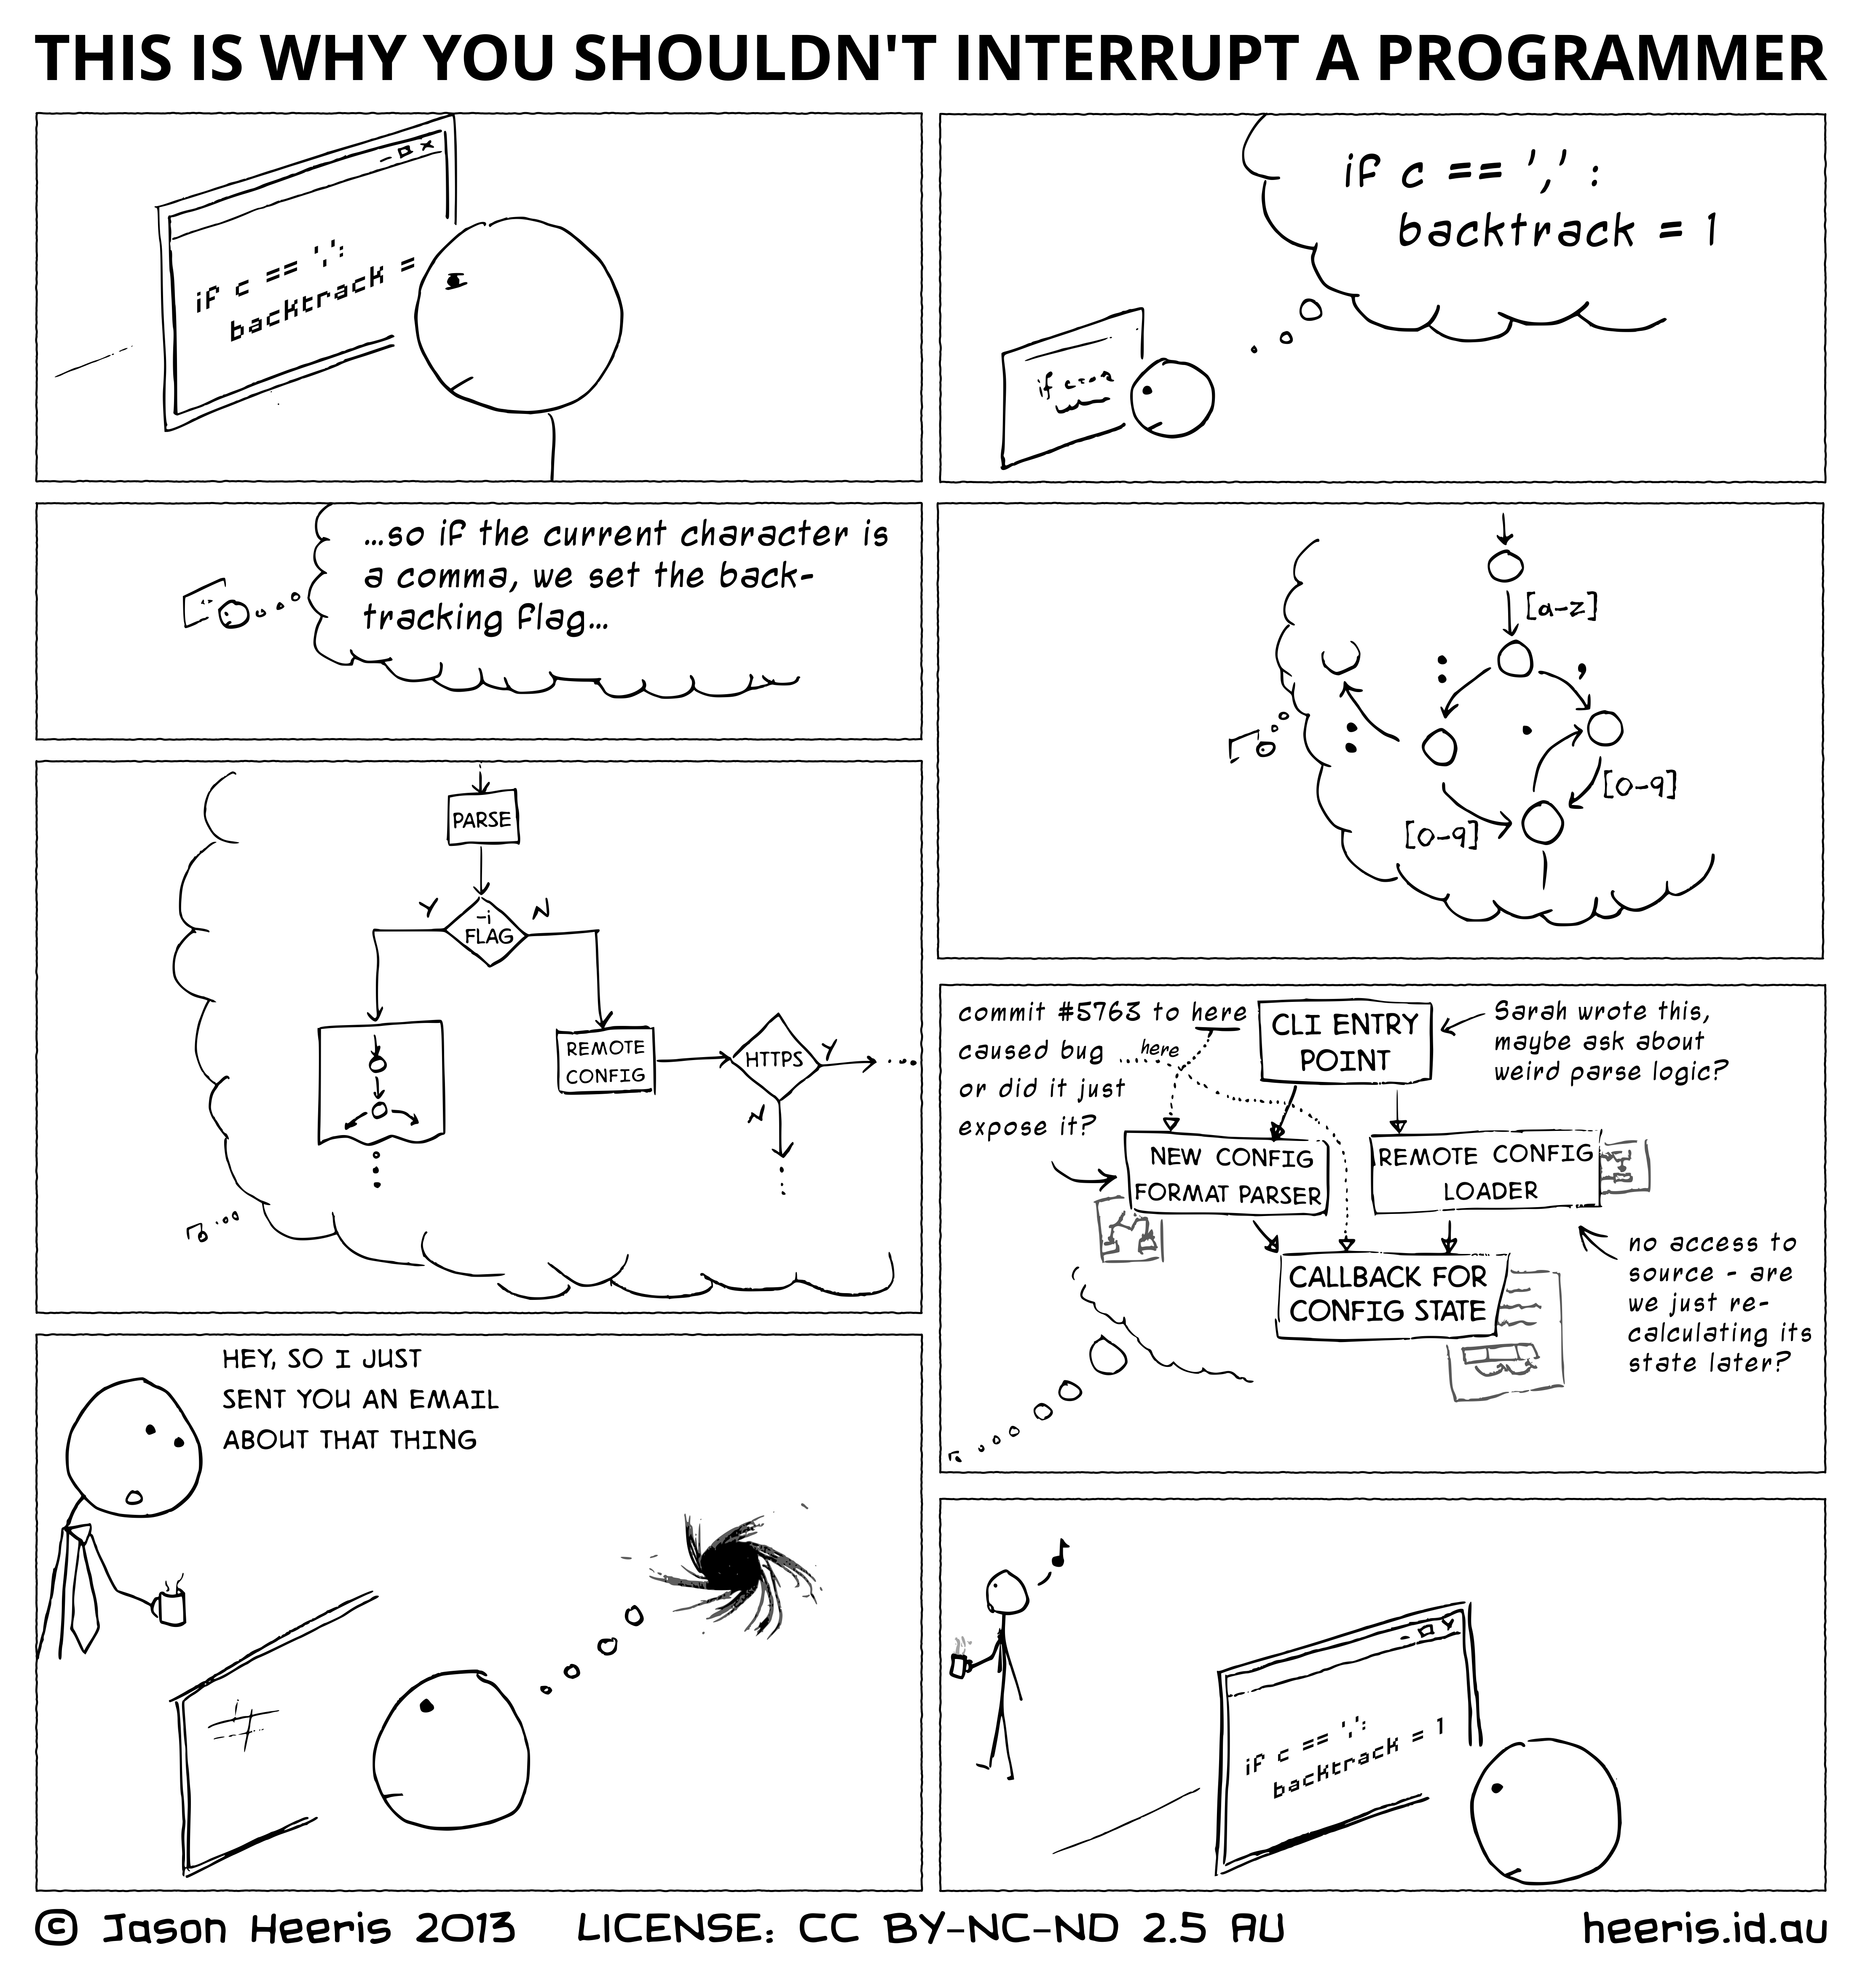
\includegraphics[scale=0.117]{data/ProgrammerInterrupted.png}}
\cite{programmerInterrupted}
\end{figure}  

\chapter{AnyOffice}\label{anyoffice}
\pict{AnyOffice - Profile}{data/anyoffice_personEdit.png}{width=1\textwidth}{pic:anyofficeProfile}
\pict{AnyOffice - Home page}{data/anyoffice_home.png}{width=1\textwidth}{pic:anyofficeHome}
\pict{AnyOffice - Graph of States}{data/anyoffice_graph.png}{width=1\textwidth}{pic:anyofficeGraph}
\pict{AnyOffice - FAQ}{data/anyoffice_faq.png}{width=1\textwidth}{pic:anyofficeFaq}
\pict{AnyOffice - Client Application}{data/client.png}{width=0.5\textwidth}{pic:anyofficeClient}
\pict{AnyOffice - Packages}{data/packages.png}{height=1\textheight}{pic:anyofficePackages}

\chapter{Contents of the Attached CD}
The CD attached at the back cover of the thesis contains:
\begin{itemize}
	\item the source code of the application;
	\item the web application packed into a \texttt{war} file ready to be deployed
	\item the client application in a form of a runnable jar 
\end{itemize}
Note, that the applications are pre-configured for the use in Y Soft Corporation. See section \ref{deployment} for more information on the deployment of the applications.


\end{document}